\documentclass[11pt,fleqn]{article} 
\usepackage[margin=0.8in, head=0.8in]{geometry} 
\usepackage{amsmath, amssymb, amsthm}
\usepackage{fancyhdr} 
\usepackage{palatino, url, multicol}
\usepackage{graphicx, pgfplots} 
\usepackage[all]{xy}
\usepackage{polynom,tabularx} 
%\usepackage{pdfsync} %% I don't know why this messes up tabular column widths
\usepackage{enumerate, adjustbox}
\usepackage{framed}
\usepackage{setspace}
\usepackage{array}
\usepackage{pgf,tikz}
\usepackage{mathrsfs}

\usepackage[parfill]{parskip}
\usetikzlibrary{arrows}

\usetikzlibrary{calc}

\pgfplotsset{compat=1.6}

\pgfplotsset{soldot/.style={color=blue,only marks,mark=*}} \pgfplotsset{holdot/.style={color=blue,fill=white,only marks,mark=*}}

\renewcommand{\headrulewidth}{0pt}
\newcommand{\blank}[1]{\rule{#1}{0.75pt}}
\newcommand{\bc}{\begin{center}}
\newcommand{\ec}{\end{center}}
\newcommand{\be}{\begin{enumerate}}
\newcommand{\ee}{\end{enumerate}}

\def\ds{\displaystyle}

\renewcommand{\d}{\displaystyle}

\newcommand{\ans}[1][2]{ \ \rule{#1 in}{.5 pt} \ }


\pagestyle{fancy} 
\rfoot{5-3}

\begin{document}

\vspace*{-0.7in}

\begin{center}
  \Large\sc{Section 5.3: The Fundamental Theorem of Calculus}
  \end{center}
\begin{enumerate}
\item Let $f(x)$ be given by the graph below and define $\displaystyle{A(x) = \int_0^x f(t)dt}$.

\begin{tabular}{cc}
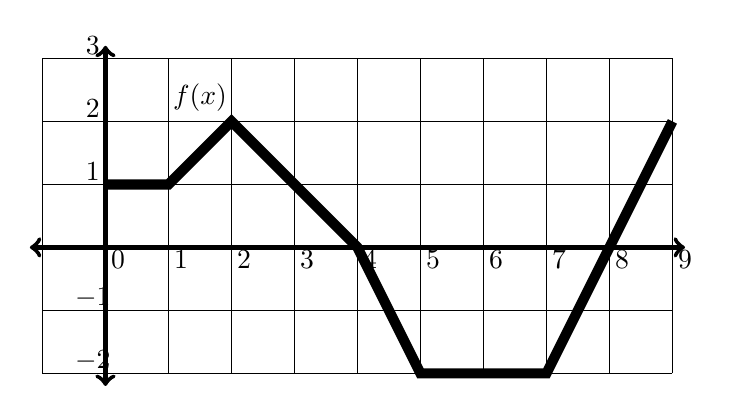
\begin{tikzpicture}[scale=.8]
\draw[<->, ultra thick](-1.2,0) -- (9.2,0);
\foreach \i in {0,1,...,9}{\node at (\i+.2,-.2){$\i$};}
\draw[<->,ultra thick](0,-2.2) -- (0,3.2);
\foreach \i in {-2,-1,1,2,3}{\node at (-.2, \i+0.2){$\i$};}
\draw[thin] (-1,-2) grid (9,3);
\draw[line width=1.3mm] (0,1) -- (1,1) -- (2,2) --(4,0)-- (5,-2)--(7,-2) -- (8,0) -- (9,2);
\draw (1.5,2) node[above] {$f(x)$};
\end{tikzpicture}
&
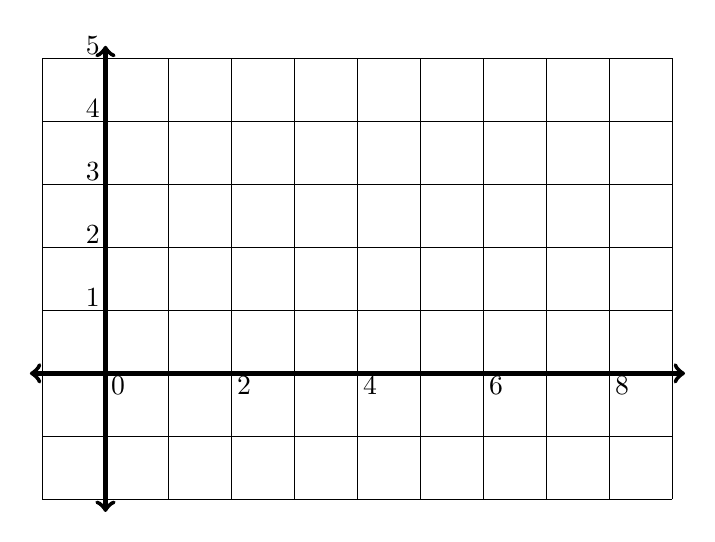
\begin{tikzpicture}[scale=.8]
\draw[<->, ultra thick](-1.2,0) -- (9.2,0);
\foreach \i in {0,2,4,6,8}{\node at (\i+.2,-.2){$\i$};}
\draw[<->,ultra thick](0,-2.2) -- (0,5.2);
\foreach \i in {1, ..., 5}{\node at (-.2, \i+0.2){$\i$};}
\draw[thin] (-1,-2) grid (9,5);
\end{tikzpicture}
\end{tabular}

\begin{enumerate}
\item Compute the following using the graph of $f(x)$. Then sketch $A(x).$

\renewcommand{\baselinestretch}{3}
\begin{multicols}{4}

\renewcommand{\baselinestretch}{3}
$f(0) = $\hrulefill
\vfill
$f(1) = $\hrulefill
\vfill

$f(2) = $\hrulefill
\vfill

$f(3) = $\hrulefill
\vfill

$f(4) = $\hrulefill

$f(5) = $\hrulefill

$f(6) = $\hrulefill

$f(7) = $\hrulefill

$f(8) = $\hrulefill

$f(9) = $\hrulefill

$A(0) =$ \hrulefill

\vfill

$A(1) =$ \hrulefill

\vfill
$A(2) = $\hrulefill
\vfill

$A(3) =$ \hrulefill
\vfill

$A(4) = $\hrulefill
\vfill

$A(5) = $\hrulefill
\vfill

$A(6) = $\hrulefill
\vfill

$A(7) = $\hrulefill
\vfill

$A(8) = $\hrulefill
\vfill

$A(9) = $\hrulefill
\vfill


\end{multicols}

\vfill

\item  Where is $A(x)$ increasing? \hrulefill
\vfill

\item Describe $f$ when $A(x)$ is increasing. \hrulefill
\vfill

\item Where is $A(x)$ decreasing? \hrulefill
\vfill

\item Describe $f$ when $A(x)$ is decreasing. \hrulefill
\vfill

\item Where does $A(x)$ have a local maximum? \hrulefill
\vfill

\item Describe $f$ when $A(x)$ has a local max. \hrulefill
\vfill

\item Where does $A(x)$ have a local minimum? \hrulefill
\vfill

\item Describe $f$ when $A(x)$ has a local min. \hrulefill

\vfill
\item What can you say about the {\bf rate of change} of $A(x)$? 
\vfill
\end{enumerate}
\newpage
\item The Fundamental Theorem of Calculus (part 1):
\vfill
\item Find the derivative of each function below.
	\begin{multicols}{2}
	\begin{enumerate}
	\item $\d g(x)=\int_2^x (t^2-\tan (t) ) \: dt$
	\item $\d h(x)=\int_0^{\sin(x)} \sqrt{t^3+1} \: dt$
	\end{enumerate}
	\end{multicols}
\vfill
\item The Fundamental Theorem of Calculus (part 2):
\vfill
\item Evaluate the integrals.
	\begin{multicols}{2}
	\begin{enumerate}
	\item $\d g(x)=\int_0^{\pi} \sin (x) \: dx$
	\item $\d h(x)=\int_{-1}^3 x+e^x \: dx$
	\end{enumerate}
	\end{multicols}
\vfill


\end{enumerate}
\end{document}
